%\documentclass[fleqn, letterpaper]{amsart}
\documentclass[fleqn, letterpaper]{tufte-handout}
\usepackage{times}
\usepackage{amsmath}
\usepackage{graphicx}
\usepackage{booktabs}
\usepackage{multirow}
%\usepackage[left=1in]{geometry}

\newcommand{\R}{\mathcal{R}}
\newcommand{\E}{\text{E}}
\newcommand{\p}{p_{XY}}
\renewcommand{\arraystretch}{1.5}

\title{Problem Set 2 --- ENCE689E Spring 2014}
\author{David Prentiss}

\begin{document}
\maketitle


\section{1. Pairs of Random Variables: Joint PDFs}
\[
        p_{XY} = \frac{6}{5}(x+y^2)
\]
\subsection{(a)} The marginal densities are given as
\[
        p_X = \int_y \p\ dy = \int_0^1 \frac{6}{5}(x+y^2)\ dy = \frac{6}{5}(xy+\frac{y^3}{3})\bigg|_0^1
        = \frac{6}{5}(x+\frac{1}{3})
\]
\[
        p_Y = \int_x \p\ dx = \int_0^1 \frac{6}{5}(x+y^2)\ dx = \frac{6}{5}(\frac{x^2}{2}+xy^2)\bigg|_0^1
        = \frac{6}{5}(y^2+\frac{1}{2})
\]
The variables are \emph{not} independent since
\[
        p_X\cdot p_Y = \frac{1}{25}\left(36xy^2+18x+12y^2+6\right)\neq \frac{6}{5}(x+y^2) \implies
        p_X\cdot p_Y \neq \p
\]
\subsection{(b)}
\[
        p_{Y|X}(y|x) = \frac{\p}{p_X}=\frac{x+y^2}{x+\frac{1}{3}}
\]
\[
        p_{X|Y}(x|y) = \frac{\p}{p_Y}=\frac{x+y^2}{y^2+\frac{1}{2}}
\]
\subsection{(c)}
\[
        \E X= \int_0^1\int_0^1 x\p\ dx\ dy
        = \int_0^1 xp_X\ dx
        = \int_0^1 \frac{6}{5}(x^2+\frac{x}{3})\ dx
        = \frac{3}{5} \approx 0.6
\]
\[
        \E Y= \int_0^1\int_0^1 x\p\ dx\ dy
        = \int_0^1 yp_Y\ dy
        = \int_0^1 \frac{6}{5}(y^3+\frac{y}{2})\ dy
        = \frac{1}{2} = 0.5
\]
\subsection{(d)}
The correlation coefficient
\[
        E[XY] = \int_0^1\int_0^1 xy\p\ dx\ dy
        = \int_0^1\int_0^1 \frac{6}{5}(x^2y + xy^3)\ dx\ dy
        = \int_0^1\frac{1}{5}(2y + 3y^3)\ dy
        = \frac{7}{20} \approx 0.35
\]
\subsection{(e)}
\[
        \Pr(x> 0.5|y=0.5)
        = 1 - \Pr(x\leq 0.5|y=0.5)
        = 1 - \int_0^{0.5} p_{X|Y}(x|y=0.5)\ dx
        = 1 - \int_0^{0.5} \frac{1}{3}(4x+1)\ dx
        = 1 - \frac{1}{3} \approx 0.66
\]
\subsection{(f)}
\[
        \E[Y|x=0.25]
        = \int_0^1 yp_{Y|X}(y|x = 0.25)\ dy
        = \int_0^1 y\frac{\frac{1}{4}+y^2}{\frac{1}{4}+\frac{1}{3}}\ dy
        = \frac{9}{14} \approx 0.64
\]
\section{2. Linear Algebra Review}
\subsection{(a)}
\[
8C-5D = \left(\begin{array}{ccc} 0 & 0 & 40\\ 0 & 32 & -16\\ 8 & 24 & 16 \end{array}\right)
- \left(\begin{array}{ccc} 30 & -10 & 10\\ 40 & 15 & 10\\ 5 & 25 & -45 \end{array}\right)
=\left(\begin{array}{ccc} -30 & 10 & 30\\ -40 & 17 & -26\\ 3 & -1 & 61 \end{array}\right)
\]
\subsection{(b)}
\[
a^TC = \left(\begin{array}{ccc} 2 & 0 & -1 \end{array}\right)
\left(\begin{array}{ccc} 0 & 0 & 5\\ 0 & 4 & -2\\ 1 & 3 & 2 \end{array}\right)
= \left(\begin{array}{ccc} -1 & -3 & 8 \end{array}\right)
\]
\subsection{(c)}
\[
Cb = 
\left(\begin{array}{ccc} 0 & 0 & 5\\ 0 & 4 & -2\\ 1 & 3 & 2 \end{array}\right)
\left(\begin{array}{c} 6\\ -4\\ 3 \end{array}\right) =
\left(\begin{array}{c} 15\\ -22\\ 0 \end{array}\right)
\]
\subsection{(d)}
\[
D^TC^T =
\left(\begin{array}{ccc} 6 & 8 & 1\\ -2 & 3 & 5\\ 2 & 2 & -9 \end{array}\right)
\left(\begin{array}{ccc} 0 & 0 & 1\\ 0 & 4 & 3\\ 5 & -2 & 2 \end{array}\right)
=\left(\begin{array}{ccc} 5 & 30 & 32\\ 25 & 2 & 17\\ -45 & 26 & -10 \end{array}\right)
\]
\subsection{(e)}
\[
CC^T=
\left(\begin{array}{ccc} 0 & 0 & 5\\ 0 & 4 & -2\\ 1 & 3 & 2 \end{array}\right)
\left(\begin{array}{ccc} 0 & 0 & 1\\ 0 & 4 & 3\\ 5 & -2 & 2 \end{array}\right)
=\left(\begin{array}{ccc} 25 & -10 & 10\\ -10 & 20 & 8\\ 10 & 8 & 14 \end{array}\right)
\]
\subsection{(f)}
\[
DCab^T=
\left(\begin{array}{ccc} 6 & -2 & 2\\ 8 & 3 & 2\\ 1 & 5 & -9 \end{array}\right)
\left(\begin{array}{ccc} 0 & 0 & 5\\ 0 & 4 & -2\\ 1 & 3 & 2 \end{array}\right)
\left(\begin{array}{c} 2\\ 0\\ -1 \end{array}\right)
\left(\begin{array}{ccc} 6 & -4 & 3 \end{array}\right)
= \left(\begin{array}{ccc} -204 & 136 & -102\\ -204 & 136 & -102\\ 30 & -20 & 15 \end{array}\right)
\]
\subsection{(g)}
\[ab^T=
\left(\begin{array}{c} 2\\ 0\\ -1 \end{array}\right)
\left(\begin{array}{ccc} 6 & -4 & 3 \end{array}\right)
=\left(\begin{array}{ccc} 12 & -8 & 6\\ 0 & 0 & 0\\ -6 & 4 & -3 \end{array}\right)
\]
\section{3. Gaussian Random Vectors and Evolving PDFs}
\subsection{(a)}
The standard deviations are the square roots of the diagonal of $Cyy$. They are 3 and 5 for $y_{1t}$ and $y_{2t}$ respectively.
\subsection{(b)}
\[
        \rho_{yy} = \frac{10}{3\cdot5} = \frac{2}{3}
\]
\subsection{(c)}
\begin{figure*}[h!]
        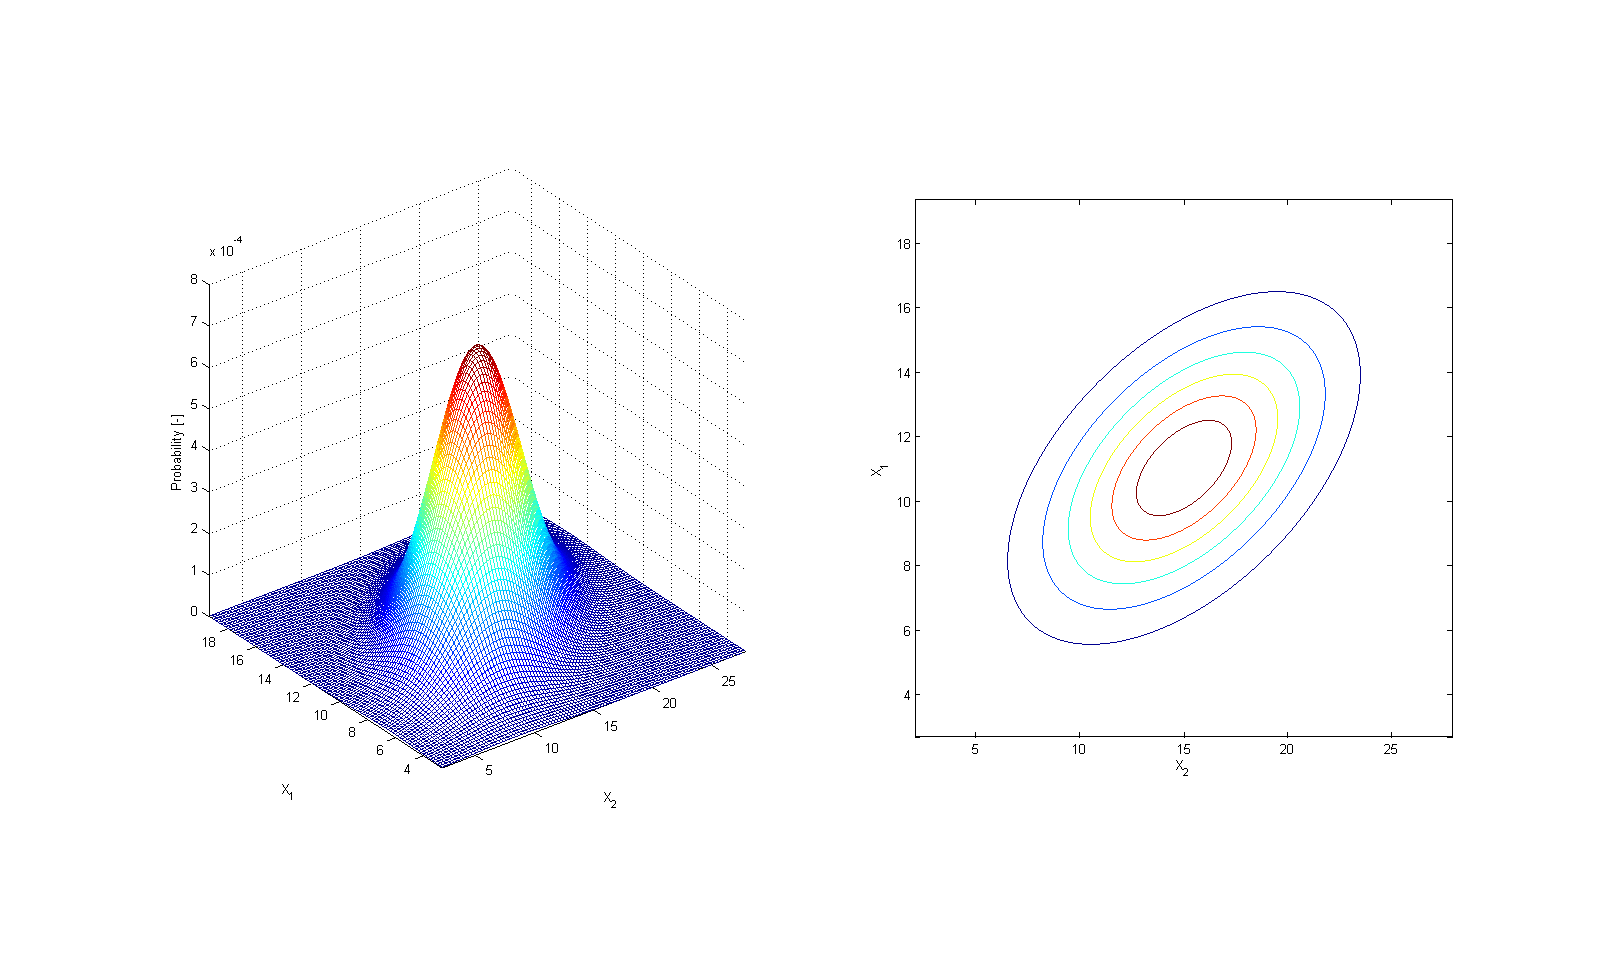
\includegraphics[width=\textwidth]{ps2plot}
\end{figure*}
\subsection{(d)}
Since the $y_t$ and $u_t$ are Guassian and $y_{t+1}$ is a linear transformation, $y_{t+1}$ is also Gaussian.
\subsection{(e)}
From the lecture notes, the mean vector of $y_{t+1}$ is
\[A\bar y_t + G\bar u_t + b
\]
\subsection{(f)}
From the lecture notes, the covariance matrix of $y_{t+1}$ is
\[AC_{yy}A^T + GC_{uu}G^T
\]
\subsection{(g)}
The mean and  covariance of $y_{t+1}$ are, respectively
\[
\left(\begin{array}{c} 11\\ 15 \end{array}\right),\ 
\left(\begin{array}{cc} \frac{387}{50} & \frac{1259}{200}\\ \frac{1259}{200} & \frac{7369}{400} \end{array}\right)
\]
The standard deviations are 2.7821 and 4.2921 for $y_{1,t+1}$ and $y_{2,t+2}$ respectively. The correlation coefficient is 0.5272. See the following code:
\begin{verbatim}
%-- 2/18/2014 8:07 PM --%
yt = [10; 15];
Cyy = [9 10; 10 25];
A = [.9 -.1;.2 .75];
G = eye(2,2);
u = [3; 1];
Cuu = [2 0; 0 1];
b = [0.50; 0.75];
yt1 = A*yt + G*u + b;
Cyy1 = A*Cyy*A' + G*Cuu*G';
plot_bivar_norm(yt1,Cyy1);    % plot yt1
sd1 = sqrt(Cyy1(1,1));        % standard deviation yt1
sd2 = sqrt(Cyy1(2,2));        % standard deviation yt2
rho1 = Cyy1(1,2)/(sd1 * sd2); % correlation coefficient
\end{verbatim}
\subsection{(h)}
\begin{figure*}[h!]
        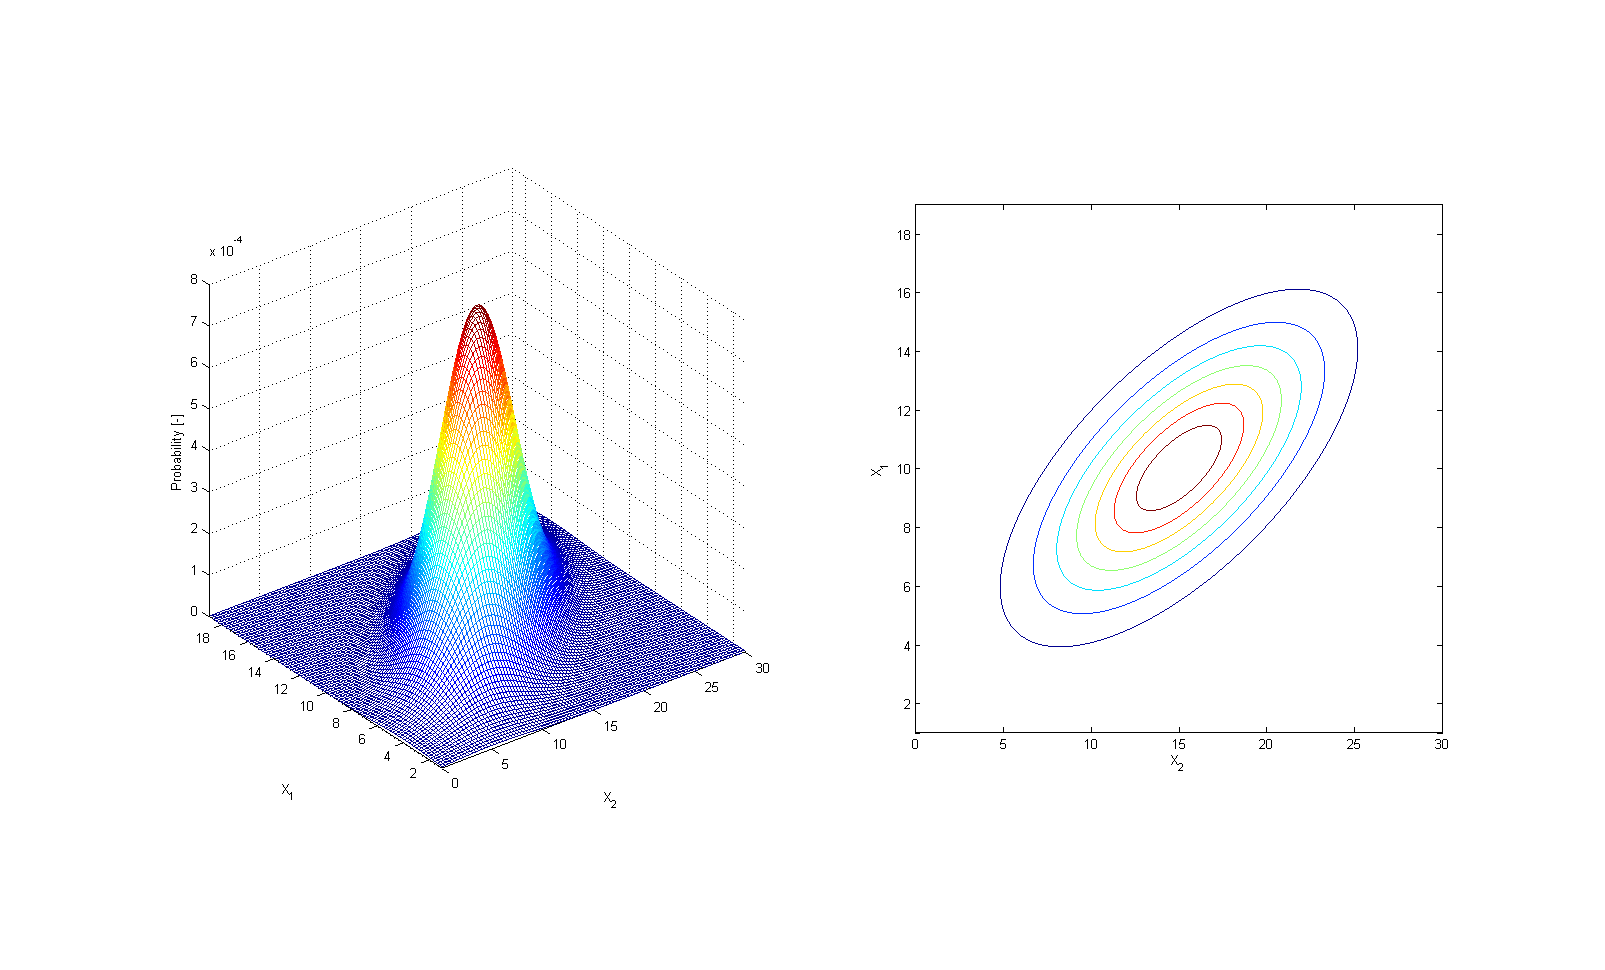
\includegraphics[width=\textwidth]{ps2plot2}
\end{figure*}
\end{document}
